\documentclass[a4paper]{article}
\usepackage[top=13.5mm, bottom=13.5mm, left=10mm, right=10mm]{geometry}
\usepackage{tikz}

\begin{document}
\thispagestyle{empty} % No page numbers

\noindent % Prevents extra spacing that could cause a new page
\begin{center}
    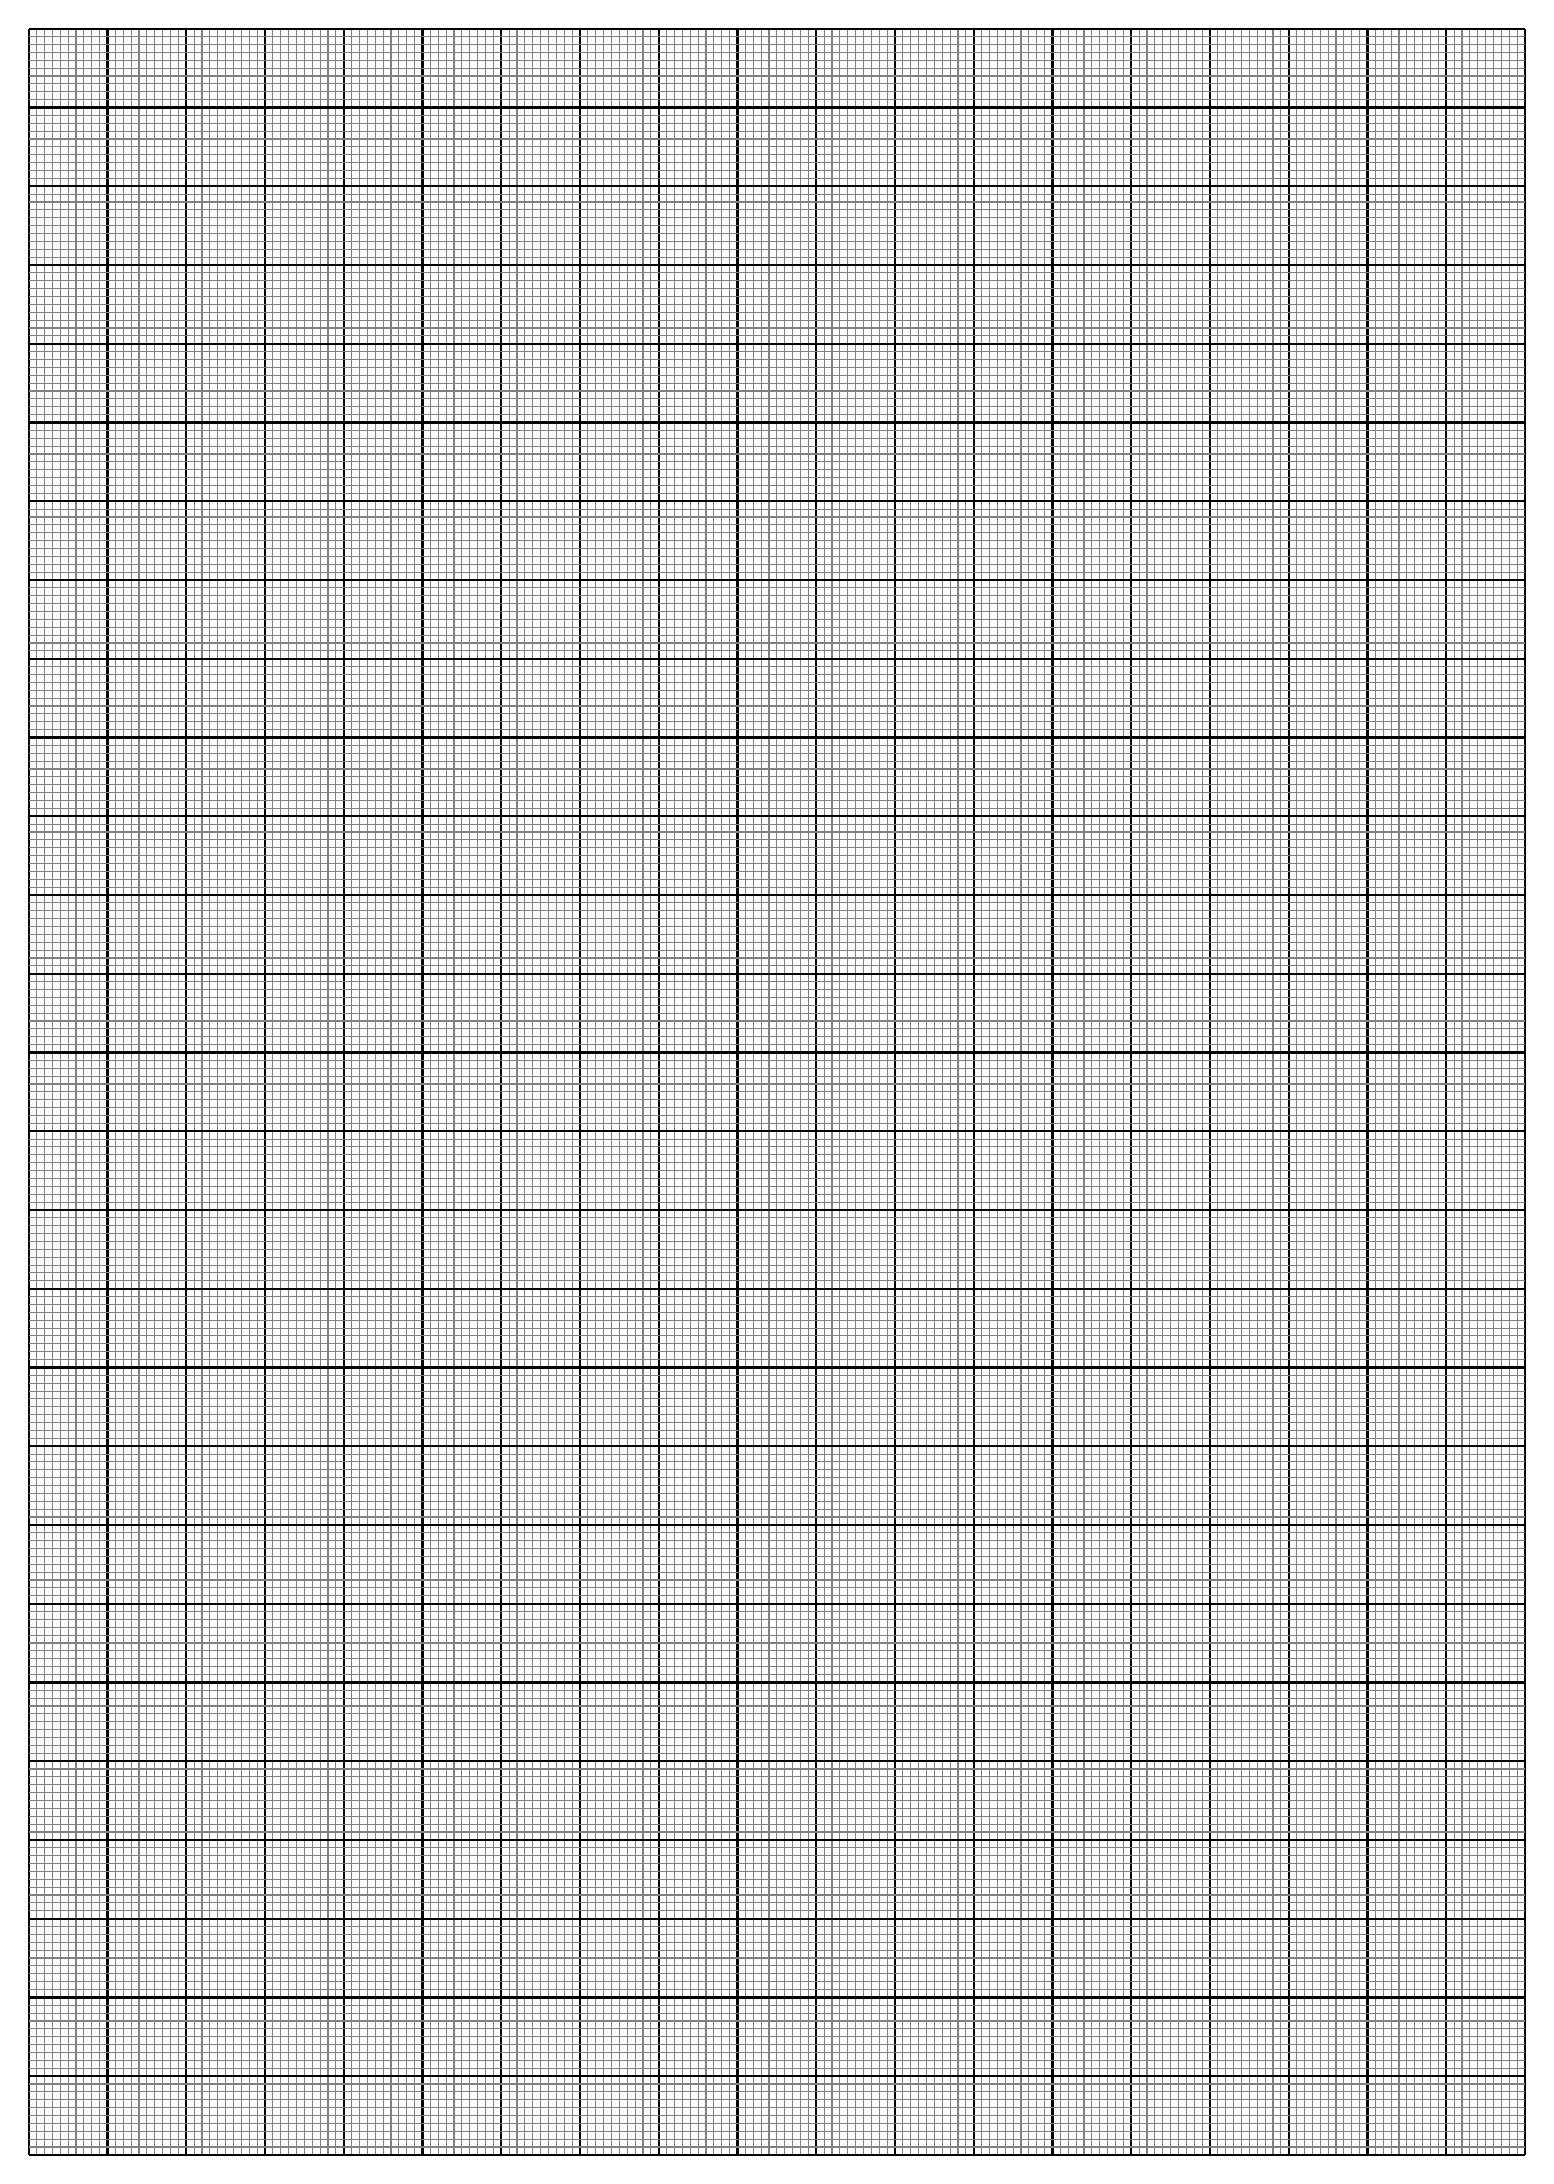
\begin{tikzpicture}[scale=0.1] % Scale to match mm units
        % Define usable area in millimeters
        \def\pageWidth{190}  % 210 - 10 - 10
        \def\pageHeight{270} % 297 - 13.5 - 13.5

        % Draw vertical grid lines every 1mm
        \foreach \x in {0,1,...,190} {
            \draw[thin,gray] (\x, 0) -- (\x, \pageHeight);
        }
        
        % Draw bold vertical lines every 10mm
        \foreach \x in {0,10,...,190} {
            \draw[thick,black] (\x, 0) -- (\x, \pageHeight);
        }

        % Draw horizontal grid lines every 1mm
        \foreach \y in {0,1,...,270} {
            \draw[thin,gray] (0, \y) -- (\pageWidth, \y);
        }
        
        % Draw bold horizontal lines every 10mm
        \foreach \y in {0,10,...,270} {
            \draw[thick,black] (0, \y) -- (\pageWidth, \y);
        }

    \end{tikzpicture}
\end{center}

\end{document}
